% Chapter 10 -- translated by Claude (2026), continuing the voice and
% register of the Burkett-Hutcheson chapters.

\chapter{Simulation in the frequency domain}

\section{Door for the frequency domain: fd}

To run a simulation in the complex frequency domain $s$, the door
called \code{sq\char`\\fd} is used.

\section{Input data}

The only input data that must be given to this door is the circuit
description, using the same notation we have seen so far. There is a
single difference: if the circuit to be simulated has any inductor
or capacitor, then the description of each element must have five
terms. Descriptions that only require four terms must have a 0 at
the end, to keep the symmetry. The frequency domain simulation is
ordered like this: \code{sq\char`\\fd(circuit)}.

\section{Initial conditions}

The fifth term in the description of an inductor or a capacitor is
its initial condition. Initial means at time $t = 0^{+}$.

The initial condition of an inductor is its initial current, and
therefore its value must be given in amperes. This current is
considered as flowing through the element from the first node to the
second node of the description.

The initial condition of a capacitor is its initial voltage, and
therefore its value must be given in volts. This voltage is
considered as the voltage of the first node with respect to the
second node of the description.

If the circuit does not specify the initial condition of the element
nor provides means to obtain it, its initial condition is assumed to
be null, that is, 0.

\section{Answers}

In the case of the frequency domain simulation, the answers are: the
node voltages, the voltage drops in the elements and the currents in
the elements. The powers consumed by the elements are not given.
There is one difference: the answers will be symbolic expressions as
functions of the complex frequency $s$.

\section{Transfer function}

Problems that ask us to find the transfer function, $H(s)$, are very
common when studying analysis in the complex frequency domain. In
the case that the problem only gives us the passive network whose
transfer function we want to find, we must add a source at the
input, preferably a current source with a symbolic or unit value.

Let us see some examples.

\problem{068}

\emph{Problem: Find $H(s) = V_{out}/V_{in}$ for the network of the
figure, and locate all its critical frequencies.}


% figures added 10 Sep 2026
\begin{figure}[!ht]
\centering
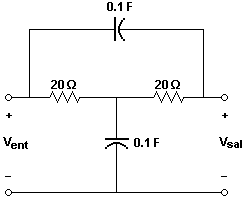
\includegraphics[width=83mm]{book_figures/p068_0.png}
\caption*{Circuit for Problem 068}
\end{figure}

Solution: We add a source, and order the simulation. Note that we
use five terms per element:

\begin{entry}
sq\fd("j1,0,1,1,0;r1,1,2,20,0;r2,2,3,20,0;ca,1,3,.1,0;
      cb,2,0,.1,0")
\end{entry}

With \key{ENTER}, the simulation executes. We request the transfer
function \code{v3/v1} and obtain
\code{(s\^{}2+s+.25)/(s\^{}2+1.5*s+.25)}. To find the critical
frequencies, that is, the poles and zeros, we will use a calculator
command.

\section{Poles, zeros and the zeros command}

The calculator has a command called \code{zeros}, which allows
finding the zeros of a polynomial, for a given variable. It is used
like this:

\begin{entry}
zeros(polynomial,variable)
\end{entry}

The complex version of this command is another command called
\code{cZeros}, which is used the same way.

We can find the zeros of a transfer function using this command,
like this: \code{zeros(}transfer function\code{)}. We can find the
poles of a transfer function using this command, like this:
\code{zeros(}inverse of the transfer function\code{)}. The inverse
of the transfer function is 1 over the function, or the function
raised to $-1$.

Let us solve the second question of the problem. We request the
zeros like this: \code{zeros(v3/v1,s)} and obtain \code{\{-1/2\}}.
Although the command does not tell us so, this is a double zero. We
request the poles like this: \code{zeros(v1/v3,s)} and obtain
\code{\{-1.31,-.191\}}. So, we have finished our first problem in
the frequency domain.

\problem{069}

\emph{Problem: Find $H(s) = V_o/V_s$ for the circuit of the
figure.}


% figures added 10 Sep 2026
\begin{figure}[!ht]
\centering
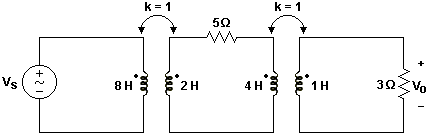
\includegraphics[width=146mm]{book_figures/p069_0.png}
\caption*{Circuit for Problem 069}
\end{figure}

Solution: There is no need to add a source, because the circuit
includes one. We order the simulation, using five terms per element,
and giving the value of the mutual inductances as $M$ instead of
$k$:

\begin{entry}
sq\fd("es,1,0,vs,0;l1,1,0,8,0;l2,2,0,2,0;r1,2,3,5,0;
      l3,3,0,4,0;l4,4,0,1,0;r2,4,0,3,0;
      m1,l1,l2,√(8*2),0;m2,l3,l4,√(4*1),0")
\end{entry}

With \key{ENTER}, the simulation executes. We request the transfer
function \code{v4/v1} and obtain \code{3*s/(17*s+15)}. Let us now
see an example of greater difficulty, but first let us learn a new
concept.

\section{Exact vs approximate}

In section 2.9 we learned that there are two ways in which the
calculator can handle a number: as exact and as approximate. What
determines which mode the calculator will use to solve a circuit is
the way in which the data is entered. Let us see the advantages and
disadvantages of each of these two modes.

\emph{Exact mode:}

Disadvantage: generally, the solution of the equations takes more
time.

Advantage: some systems of equations can be solved precisely that in
approximate mode could turn out to be unsolvable, or solved
imprecisely.

\emph{Approximate mode:}

Advantage: generally, the solution of the equations takes less time.

Disadvantage: in some particular cases, it is possible that a system
of equations cannot be solved in this mode, even though in exact
mode it would have been solved. In other particular cases, it is
possible that the answers lose precision, especially in the case of
large numbers.

In the great majority of cases, either of the two modes can be used
interchangeably. However, when dealing with large circuits, it is
preferable to choose the mode that best fits our need.

\problem{070}

\emph{Problem: Find $H(s) = V_{out}/V_{in}$ for the network of the
figure. The op-amps are ideal.}


% figures added 10 Sep 2026
\begin{figure}[!ht]
\centering
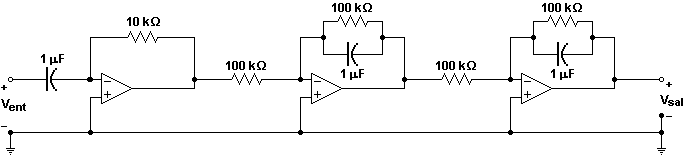
\includegraphics[width=150mm]{book_figures/p070_0.png}
\caption*{Circuit for Problem 070}
\end{figure}

Solution: We order the simulation, using five terms per element. We
prefer to use all the values in exact form, to guarantee the best
probability of obtaining a solution, regardless of the solution
time:

\begin{entry}
sq\fd("e1,1,0,1,0;cc1,1,2,10^-6,0;r1,2,3,10^4,0;o1,0,2,3,0;
      r2,3,4,10^5,0;r3,4,5,10^5,0;cc2,4,5,10^-6,0;o2,0,4,5,0;
      r4,5,6,10^5,0;r5,6,7,10^5,0;cc3,6,7,10^-6,0;o3,0,6,7,0")
\end{entry}

With \key{ENTER}, the simulation executes. This simulation takes
more time than any we have seen so far. This increase in time is due
not only to the generated equations being enormous, but to the limit
being applied to all the answers, since there are op-amps in the
circuit. When ordering this simulation, you can leave the calculator
executing it and go have lunch. When you return, you will find that
the simulation has finished. We request the transfer function
\code{v7/v1} and obtain the expression \code{-s/(s+10)\^{}2}.

Here a note must be made. A numerical simulator, such as SPICE,
could find the numerical value of the output voltage, if we give it
a numerical value for the input voltage and a numerical value for
the frequency. But to obtain a symbolic expression for the transfer
function, in terms of $s$, it is necessary to use a symbolic
simulator, like Symbulator.

Let us now see four examples that illustrate that the
\code{thevenin} tool can also be used in the complex frequency
domain.

\problem{071}

\emph{Problem: Find: a) $Z_{in}$ for the network of the figure, in
terms of $s$, b) $Z_{in}(j8)$ in rectangular form, c)
$Z_{in}(-2+j6)$ in polar form, d) to what value the 16~$\Omega$
resistor must be changed so that $Z_{in} = 0$ at $s = -5 + j0$, e)
to what value the 16~$\Omega$ resistor must be changed so that
$Z_{in} = \infty$ at $s = -5 + j0$.}


% figures added 10 Sep 2026
\begin{figure}[!ht]
\centering
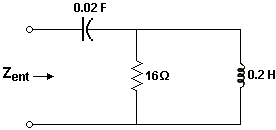
\includegraphics[width=94mm]{book_figures/p071_0.png}
\caption*{Circuit for Problem 071}
\end{figure}

Solution: We execute the tool, using five terms per element:

\begin{entry}
sq\thevenin("c,1,2,.02,0;r,2,0,16,0;l,2,0,.2,0",1,0)
\end{entry}

We press \key{ENTER}. We choose Passive and FD. We press
\key{ENTER}. We answer question a) in this first step. We see on the
screen the value of \code{zth}. We exit with \key{ENTER}. We can
request \code{zth} and obtain the expression
\code{16.*(s\^{}2+3.125*s+250.)/(s*(s+80.))}.

We answer question b) like this: \code{zth|s=8i→Rect} and obtain
$.158 - 4.67i$.

We answer question c) like this:
\code{sq\char`\\absang(zth|s=-2+6i)} and obtain 6.85∠$-$114.°.

To answer the two following questions, we simulate again, using a
symbolic value for the resistor:

\begin{entry}
sq\thevenin("c,1,2,.02,0;r,2,0,r,0;l,2,0,.2,0",1,0)
\end{entry}

With \key{ENTER}, the tool executes. We choose Passive and FD. We
press \key{ENTER}. We see on the screen the value of \code{zth}. We
exit with \key{ENTER}. We answer question d) like this:
\code{cSolve(zth=0,r)|s=-5} and obtain \code{r}~$= .909$.

To answer question e), we require two steps:

\begin{entry}
cSolve(zth=x,r)|s=-5
\end{entry}

We obtain \code{r=(x+10.)/(x+11.)}. Now the second step:

\begin{entry}
limit(ans(1),x,∞)
\end{entry}

We obtain 1. This is the correct answer.

\problem{072}

\emph{Problem: This problem has no figure. A network is composed of
a 1~µF capacitor in parallel with the series combination of a 20~mH
inductor and a 500~$\Omega$ resistor. a) Find $Z_{in}(s)$ for the
network, in terms of $s$. b) If $s = \sigma - j0$, find the value of
$\sigma$, between $-20$ and $-10$~kNp/s, at which
$\mathrm{abs}(Z_{in})$ is a minimum. c) Again with
$s = \sigma - j0$, find the value of $\sigma$, smaller than
$-30$~kNp/s, at which $\mathrm{abs}(Z_{in})$ is a maximum.}

Solution: We execute the tool:

\begin{entry}
sq\thevenin("c,1,0,1E-6,0;l,1,2,.02,0;r,2,0,500,0",1,0)
\end{entry}

We press \key{ENTER}. We choose Passive and FD. We press
\key{ENTER}. We answer question a) in this first step. We see on the
screen the value of \code{zth}. We exit with \key{ENTER}. In any
case, we request it as \code{zth} and obtain the expression:

\begin{entry}
1000000.*(s+25000.)/(s^2+25000.*s+50000000.)
\end{entry}

To answer questions b) and c), we remember that both the minimum and
the maximum are points at which the slope of the graph is 0. Using
the derivative, we can solve with \code{solve} for those frequencies
at which the derivative becomes 0:

\begin{entry}
solve(d(abs(zth),s)=0,s)
\end{entry}

The \code{d} is the derivative, and is entered with the key
combination \key{2nd} \key{8}. The command means: ``Find the values
of $s$ at which the derivative of the absolute value of \code{zth}
with respect to $s$ is worth zero.'' We obtain \code{s}~$= -17929.$
or \code{s}~$= -32071.$ According to what the problem statement
tells us, the first value is a minimum and the second is a maximum.
With this, we have answered the questions.

\problem{073}

\emph{Problem: Find: a) $Z_{in}(\sigma)$ as a function of $\sigma$
for the network of the figure, b) find all the zeros and poles, c)
graph $\mathrm{abs}(Z_{in}(\sigma))$ vs $\sigma$, d) graph
$\mathrm{ang}(Z_{in}(\sigma))$ vs $\sigma$.}


% figures added 10 Sep 2026
\begin{figure}[!ht]
\centering
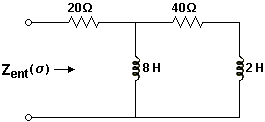
\includegraphics[width=90mm]{book_figures/p073_0.png}
\caption*{Circuit for Problem 073}
\end{figure}

% figures added 10 Sep 2026
\begin{figure}[!ht]
\centering
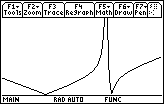
\includegraphics[width=56mm]{book_figures/p073_1.png}
\caption*{Graph requested by part (c) of Problem 073}
\end{figure}

% figures added 10 Sep 2026
\begin{figure}[!ht]
\centering
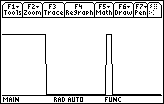
\includegraphics[width=56mm]{book_figures/p073_2.png}
\caption*{Graph requested by part (d) of Problem 073}
\end{figure}

Solution: We execute the tool:

\begin{entry}
sq\thevenin("r1,1,2,20,0;l1,2,0,8,0;r2,2,3,40,0;l2,3,0,2,0",1,0)
\end{entry}

We press \key{ENTER}. We choose Passive and FD. We press
\key{ENTER}. We see on the screen the value of \code{zth}, as a
function of $s$. We press \key{ENTER} to exit. Requesting
\code{zth|s=σ→zth} we obtain the expression
\code{4*(2*σ\^{}2+65*σ+100)/(5*(σ+4))}.

Let us answer question b). We request the zeros with
\code{zeros(zth,σ)} and obtain
\code{\{5*(√137-13)/4,-5*(√137+13)/4\}}. If we prefer to see these
zeros in approximate form, we use \key{$\diamond$} \key{ENTER} and
receive \code{\{-1.62,-30.9\}}. We request the poles with
\code{zeros(1/zth,σ)} and obtain \code{\{-4\}}.

To make the graph that question c) requests, we follow these steps:

\begin{entry}
abs(zth)|σ=x
ans(1)→y1(x)
\end{entry}

We use \code{ans(1)} because the expression is above. We press
\key{$\diamond$} \key{WINDOW}. Here we can specify the range we wish
to graph. We use \code{xmin}~$= -50$ and \code{xmax}~$= 20$. We
press \key{$\diamond$} \key{GRAPH}. The calculator graphs the
function, but using an inappropriate vertical scale. We press
\key{F2} \key{A} on the TI-89, to apply the ZoomFit command. We see
the graph, at the correct scale.

To make the graph that question d) requests, we follow these steps:

\begin{entry}
angle(zth)|σ=x
ans(1)→y1(x)
\end{entry}

We press \key{$\diamond$} \key{WINDOW}. Here we can specify the
range we wish to graph. We use \code{xmin}~$= 0$ and
\code{xmax}~$= 4$. We press \key{$\diamond$} \key{GRAPH}. The graph
appears, with an inappropriate scale. We apply the ZoomFit command.
We see the graph, at the correct scale.

So, we have answered all the questions.

\problem{074}

\emph{Problem: Find: a) $Z_{in}(s)$ for the network of the figure,
b) find all the critical frequencies, c) graph
$\mathrm{abs}(Z_{in}(s))$ vs $s$.}


% figures added 10 Sep 2026
\begin{figure}[!ht]
\centering
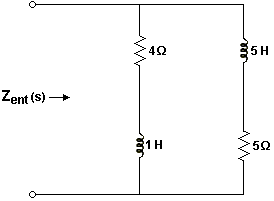
\includegraphics[width=93mm]{book_figures/p074_0.png}
\caption*{Circuit for Problem 074}
\end{figure}

% figures added 10 Sep 2026
\begin{figure}[!ht]
\centering
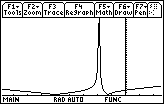
\includegraphics[width=56mm]{book_figures/p074_1.png}
\caption*{Graph requested by part (c) of Problem 074}
\end{figure}

Solution: We execute the tool:

\begin{entry}
sq\thevenin("r1,1,2,4,0;l1,2,0,1,0;l2,1,3,5,0;r2,3,0,5,0",1,0):zth
\end{entry}

We press \key{ENTER}. We choose Passive and FD. We press
\key{ENTER}. We see on the screen the value of \code{zth}, as a
function of $s$. We exit with \key{ENTER}. In the history area we
see \code{5*(s+1)*(s+4)/(3*(2*s+3))}. This expression appeared now,
because we used \code{:zth} at the end of the command line.

For question b), we request the zeros with \code{cZeros(zth,s)} and
obtain \code{\{-4,-1\}}. We request the poles with
\code{cZeros(1/zth,s)} and obtain \code{\{-3/2,-∞,∞\}}. We use the
\code{cZeros} command instead of the \code{zeros} command because,
unlike the previous problem, this time we are looking for poles in
$s$, which can be complex. So, we use the \code{cZeros} command when
we are going to find complex critical frequencies, and the
\code{zeros} command when we are going to find real critical
frequencies.

To make the graph that question c) requests, we follow these steps:

\begin{entry}
abs(zth)|s=x
ans(1)→y1(x)
\end{entry}

We use \code{ans(1)} because the expression is above. We press
\key{$\diamond$} \key{WINDOW}. Here we can specify the range we wish
to graph. We use \code{xmin}~$= -7$ and \code{xmax}~$= 2$. We press
\key{$\diamond$} \key{GRAPH}. The calculator graphs the function,
but using an inappropriate vertical scale. We press \key{F2} \key{A}
on the TI-89, to apply the ZoomFit command. We see the graph, at the
correct scale.

So, we have answered all the questions.
